
\documentclass[12pt,halfline,a4paper,]{ouparticle}

% Packages I think are necessary for basic Rmarkdown functionality
\usepackage{hyperref}
\usepackage{graphicx}
\usepackage{listings}
\usepackage{xcolor}
\usepackage{fancyvrb}
\usepackage{framed}

% Link coloring
\hypersetup{breaklinks=true,
            bookmarks=true,
            pdfauthor={},
            pdftitle={STA304XS - Assignment 1}
            }


%% To allow better options for figure placement
%\usepackage{float}

% Packages that are supposedly required by OUP sty file
\usepackage{amssymb, amsmath, geometry, amsfonts, verbatim, endnotes, setspace}

% use upquote if available, for straight quotes in verbatim environments
\IfFileExists{upquote.sty}{\usepackage{upquote}}{}

% Macros for dealing with affiliations, footnotes, etc.
\makeatletter
\def\Newlabel#1#2#3{\expandafter\gdef\csname #1@#2\endcsname{#3}}

\def\Ref#1#2{\@ifundefined{#1@#2}{???}{\csname #1@#2\endcsname}}

\newcommand*\samethanks[1][\value{footnote}]{\footnotemark[#1]}

\newcommand*\ifcounter[1]{%
  \ifcsname c@#1\endcsname
    \expandafter\@firstoftwo
  \else
    \expandafter\@secondoftwo
  \fi
}

\newcommand*\thanksbycode[1]{%
  \ifcounter{FNCT@#1}
    {\samethanks[\value{FNCT@#1}]}
    {\thanks{\Ref{FN}{#1}}\newcounter{FNCT@#1}\setcounter{FNCT@#1}{\value{footnote}}}
}

% Create labels for Addresses if the are given in Elsevier format

% Create labels for Footnotes if the are given in Elsevier format

% Part for setting citation format package: natbib

% Part for setting citation format package: biblatex

% Pandoc syntax highlighting
\usepackage{color}
\usepackage{fancyvrb}
\newcommand{\VerbBar}{|}
\newcommand{\VERB}{\Verb[commandchars=\\\{\}]}
\DefineVerbatimEnvironment{Highlighting}{Verbatim}{commandchars=\\\{\}}
% Add ',fontsize=\small' for more characters per line
\usepackage{framed}
\definecolor{shadecolor}{RGB}{248,248,248}
\newenvironment{Shaded}{\begin{snugshade}}{\end{snugshade}}
\newcommand{\AlertTok}[1]{\textcolor[rgb]{0.94,0.16,0.16}{#1}}
\newcommand{\AnnotationTok}[1]{\textcolor[rgb]{0.56,0.35,0.01}{\textbf{\textit{#1}}}}
\newcommand{\AttributeTok}[1]{\textcolor[rgb]{0.13,0.29,0.53}{#1}}
\newcommand{\BaseNTok}[1]{\textcolor[rgb]{0.00,0.00,0.81}{#1}}
\newcommand{\BuiltInTok}[1]{#1}
\newcommand{\CharTok}[1]{\textcolor[rgb]{0.31,0.60,0.02}{#1}}
\newcommand{\CommentTok}[1]{\textcolor[rgb]{0.56,0.35,0.01}{\textit{#1}}}
\newcommand{\CommentVarTok}[1]{\textcolor[rgb]{0.56,0.35,0.01}{\textbf{\textit{#1}}}}
\newcommand{\ConstantTok}[1]{\textcolor[rgb]{0.56,0.35,0.01}{#1}}
\newcommand{\ControlFlowTok}[1]{\textcolor[rgb]{0.13,0.29,0.53}{\textbf{#1}}}
\newcommand{\DataTypeTok}[1]{\textcolor[rgb]{0.13,0.29,0.53}{#1}}
\newcommand{\DecValTok}[1]{\textcolor[rgb]{0.00,0.00,0.81}{#1}}
\newcommand{\DocumentationTok}[1]{\textcolor[rgb]{0.56,0.35,0.01}{\textbf{\textit{#1}}}}
\newcommand{\ErrorTok}[1]{\textcolor[rgb]{0.64,0.00,0.00}{\textbf{#1}}}
\newcommand{\ExtensionTok}[1]{#1}
\newcommand{\FloatTok}[1]{\textcolor[rgb]{0.00,0.00,0.81}{#1}}
\newcommand{\FunctionTok}[1]{\textcolor[rgb]{0.13,0.29,0.53}{\textbf{#1}}}
\newcommand{\ImportTok}[1]{#1}
\newcommand{\InformationTok}[1]{\textcolor[rgb]{0.56,0.35,0.01}{\textbf{\textit{#1}}}}
\newcommand{\KeywordTok}[1]{\textcolor[rgb]{0.13,0.29,0.53}{\textbf{#1}}}
\newcommand{\NormalTok}[1]{#1}
\newcommand{\OperatorTok}[1]{\textcolor[rgb]{0.81,0.36,0.00}{\textbf{#1}}}
\newcommand{\OtherTok}[1]{\textcolor[rgb]{0.56,0.35,0.01}{#1}}
\newcommand{\PreprocessorTok}[1]{\textcolor[rgb]{0.56,0.35,0.01}{\textit{#1}}}
\newcommand{\RegionMarkerTok}[1]{#1}
\newcommand{\SpecialCharTok}[1]{\textcolor[rgb]{0.81,0.36,0.00}{\textbf{#1}}}
\newcommand{\SpecialStringTok}[1]{\textcolor[rgb]{0.31,0.60,0.02}{#1}}
\newcommand{\StringTok}[1]{\textcolor[rgb]{0.31,0.60,0.02}{#1}}
\newcommand{\VariableTok}[1]{\textcolor[rgb]{0.00,0.00,0.00}{#1}}
\newcommand{\VerbatimStringTok}[1]{\textcolor[rgb]{0.31,0.60,0.02}{#1}}
\newcommand{\WarningTok}[1]{\textcolor[rgb]{0.56,0.35,0.01}{\textbf{\textit{#1}}}}

% tightlist command for lists without linebreak
\providecommand{\tightlist}{%
  \setlength{\itemsep}{0pt}\setlength{\parskip}{0pt}}



\usepackage{float}
\floatplacement{figure}{H}
\usepackage{caption}
\captionsetup[figure]{font=scriptsize}
\pagenumbering{gobble}
\usepackage{booktabs}

\begin{document}

\title{STA304XS - Assignment 1}

\author{%
%
% Code for old style authors field
%
% Add \and if both authors and author
%
%
% Code for new (elsevier) style author field
\name{Jing Yeh}
%
\email{\href{mailto:yhxjin001@myuct.ac.za}{yhxjin001@myuct.ac.za}}%
%
%
%
\and
\name{Saurav Sathnarayan}
%
\email{\href{mailto:sthsau001@myuct.ac.za}{sthsau001@myuct.ac.za}}%
%
%
%
%
}

\abstract{This assignment addresses Bayesian inference and posterior
distribution estimation. We derive the posterior distribution, implement
an acceptance-rejection sampling algorithm, and use the sampled
parameters to generate animal movement trajectories. The results include
posterior summaries, trajectory simulations, and final estimates for the
mean and variance of the parameter of interest.}

\date{2025-09-05}

\keywords{Bayesian inference, Posterior sampling, Acceptance-Rejection,
Animal movement}

\maketitle



\subsection{Question 1}\label{question-1}

We aim to find the posterior distribution using the following formula:\\
\[\pi(\theta|V) \propto L(\theta,V)\,\pi(\theta)\]\\
We know that \(\pi(\theta) \propto 1\), thus our posterior distribution
is just\\
\[\pi(\theta|V) \propto L(\theta,V)\]\\
From our model equation V is multi-variate normally distributed,
\(V \sim \mathcal{N}_2(a M v_{t-1}, I_2)\)

\hfill\break
Our pdf is:\\
\[f(V) = \frac{1}{\sqrt{2\pi}} e^{(-\frac{1}{2}(v_t-a\pmb Mv_{t-1})^T(v_t-a\pmb Mv_{t-1}))}\]

We can simpilfy to make it easier for further calculations\\
\[f(V) \propto e^{(-\frac{1}{2}(v_t-a\pmb Mv_{t-1})^T(v_t-a\pmb Mv_{t-1}))}\]
Focusing on the exponent:\\
\[(v_t-aMv_{t-1})^\top(v_t-aMv_{t-1}) = v_t^\top v_t -v_t^\top 2aMv_{t-1} +a^2v_{t-1}^\top M^\top Mv_{t-1} =v_t^\top v_t  -v_t^\top 2aMv_{t-1} +a^2v_{t-1}^\top v_{t-1}\]\\
The terms \(v_t^\top v_t\) and \(a^2v_{t-1}^\top v_{t-1}\) are
independent of \(\theta\) thus we can factor it out of the pdf to get:

\[f(V) \propto e^{(av_t^\top Mv_{t-1})}\] We can further simply our
exponent:\\
\[v_t^\top Mv_{t-1}=\begin{pmatrix} v_{t_1} & v_{t_2} \end{pmatrix}\begin{bmatrix}
\cos \theta & \sin \theta \\
- \sin \theta & \cos \theta
\end{bmatrix}\begin{pmatrix} v_{t-1_1} \\ v_{t-1_2} \end{pmatrix}= \cos\theta(v_{t_1} v_{t_1,1} +v_{t_2} v_{t-1_2}) +\sin\theta(v_{t_1} v_{t-1_2} -v_{t_2} v_{t-1_1}) \]

So we end up with:

\[f(V) \propto \exp\frac{\cos\theta(v_{t_1} v_{t_1,1} +v_{t_2} v_{t-1_2}) +\sin\theta(v_{t_1} v_{t-1_2} -v_{t_2} v_{t-1_1})}{2}\]\\
Our likelihood is simply:\\
\[L(\theta,V) = \prod_{t=1}^n f(V, \theta)\]\\
\[L(\theta,V)   \propto\ \exp\frac{\sum_{t=1}^n(\cos\theta(v_{t_1} v_{t_1,1} +v_{t_2} v_{t-1_2}) +\sin\theta(v_{t_1} v_{t-1_2} -v_{t_2} v_{t-1_1}))}{2}\]\\
Distributing our summation we get
\(s_1 =\sum(v_{t,1} v_{t-1_1} +v_{t_2} v_{t-1_2})\) and
\(s_2 =\sum(v_{t_1} v_{t-1_2} -v_{t_2} v_{t-1_1})\)

Therefore:
\[\pi(\theta \mid V) \propto \exp({\frac{s1 \cos \theta + s2 \sin \theta}{2}})\]

\begin{center}\rule{0.5\linewidth}{0.5pt}\end{center}

\subsection{Question 2}\label{question-2}

\begin{enumerate}
\def\labelenumi{(\alph{enumi})}
\tightlist
\item
  We aim to sample from the posterior distribution of the turning angle,
  \(\pi(\theta \mid V)\), which is proportional to
  \(\exp\big((s_1\cos\theta + s_2\sin\theta)/2\big)\) for
  \(-\pi < \theta < \pi\). Since this distribution is not standard, we
  use the \textbf{Acceptance-Rejection algorithm}. A candidate
  \(\theta^*\) is drawn from a proposal distribution \(h(\theta)\), and
  it is accepted with probability \(\gamma(\theta^*)\), which is the
  ratio of the target density to a scaled proposal density. Repeating
  this procedure produces samples approximately from
  \(\pi(\theta \mid V)\)\\
  Our formula for \(\gamma(\theta)\) is:
\end{enumerate}

\[\gamma(\theta)= \frac{\pi (\theta) g(t,\theta))}{Ch{(\theta)}}\]\\
Where \(h(\theta) \propto 3\cos(\theta)\)

\[ C = \max_\theta \frac{\pi (\theta) g(t,\theta))}{h{(\theta)}}\] We
first find the C value through differentiation: Recall that
\(s_1 =\sum(v_{t,1} v_{t-1_1} +v_{t_2} v_{t-1_2})\) and
\(s_2 =\sum(v_{t_1} v_{t-1_2} -v_{t_2} v_{t-1_1})\). We would like to
maximise
\(\exp{(\frac{s_1\cos\theta + s_2 \sin\theta - 6\cos\theta}{2})}\). For
cleanliness's sake, let's define
\(A(\theta) = \exp{(\frac{s_1\cos\theta + s_2 \sin\theta - 6\cos\theta}{2})}\)
We thus have: \[
\frac{dA}{d\theta} = \frac{-(s_1 - 6)}{2}\sin\theta A(\theta) + \frac{s_2}{2}\cos\theta A(\theta) 
\] We set this to 0 to maximise. We get:

\begin{align}
 \frac{(s_1 - 6)}{2}\sin\theta A(\theta) &= \frac{s_2}{2}\cos\theta A(\theta) \\
 (s_1 - 6) \sin\theta &= s_2 \cos\theta A(\theta)\\
 \tan\theta &= \frac{s_2}{s_1 - 6}\\
 \theta &= \arctan (\frac{s_2}{s_1 - 6})
\end{align}

We confirm our value for C using R's optimise function:

\begin{Shaded}
\begin{Highlighting}[]
\CommentTok{\#posterior, same as likelihood, since prior is constant.}
\NormalTok{posterior }\OtherTok{\textless{}{-}} \ControlFlowTok{function}\NormalTok{(theta) \{}
  \FunctionTok{exp}\NormalTok{((s1 }\SpecialCharTok{*} \FunctionTok{cos}\NormalTok{(theta) }\SpecialCharTok{+}\NormalTok{ s2 }\SpecialCharTok{*} \FunctionTok{sin}\NormalTok{(theta))}\SpecialCharTok{/}\DecValTok{2}\NormalTok{)}
\NormalTok{\}}

\CommentTok{\#candidate}
\NormalTok{h }\OtherTok{\textless{}{-}} \ControlFlowTok{function}\NormalTok{(theta) \{}
  \FunctionTok{exp}\NormalTok{(}\DecValTok{3} \SpecialCharTok{*} \FunctionTok{cos}\NormalTok{(theta))}
\NormalTok{\}}


\CommentTok{\# Manual calculation}
\NormalTok{theta\_man }\OtherTok{=} \FunctionTok{atan}\NormalTok{((s2)}\SpecialCharTok{/}\NormalTok{(s1}\DecValTok{{-}6}\NormalTok{))}
\NormalTok{C\_man }\OtherTok{=} \FunctionTok{posterior}\NormalTok{(theta\_man)}\SpecialCharTok{/}\FunctionTok{h}\NormalTok{(theta\_man)}

\CommentTok{\#gamma function}
\NormalTok{gamma }\OtherTok{\textless{}{-}} \ControlFlowTok{function}\NormalTok{(theta, C) \{}
\NormalTok{  (}\FunctionTok{posterior}\NormalTok{(theta)}\SpecialCharTok{/}\NormalTok{(}\FunctionTok{h}\NormalTok{(theta)}\SpecialCharTok{*}\NormalTok{C))}
\NormalTok{\}}
\NormalTok{ opt }\OtherTok{\textless{}{-}} \FunctionTok{optimize}\NormalTok{(}\ControlFlowTok{function}\NormalTok{(theta) }\FunctionTok{posterior}\NormalTok{(theta)}\SpecialCharTok{/}\FunctionTok{h}\NormalTok{(theta),}
                  \AttributeTok{interval =} \FunctionTok{c}\NormalTok{(}\SpecialCharTok{{-}}\NormalTok{pi, pi), }\AttributeTok{maximum =} \ConstantTok{TRUE}\NormalTok{)}
\NormalTok{C }\OtherTok{\textless{}{-}}\NormalTok{ opt}\SpecialCharTok{$}\NormalTok{objective}

\NormalTok{C}
\end{Highlighting}
\end{Shaded}

\begin{verbatim}
## [1] 3.588122e+87
\end{verbatim}

\begin{Shaded}
\begin{Highlighting}[]
\NormalTok{C\_man}
\end{Highlighting}
\end{Shaded}

\begin{verbatim}
## [1] 3.588122e+87
\end{verbatim}

We can then use the Acceptance-Rejection algorithm to create sample
draws from our posterior as below: We first notice that \(h(\theta)\) is
the kernel of the von Mises distribution. We thus generate pre-filtered
theta samples with with the r function rvonmises(). Notice that von
Mises distribution is a valid choice because \(h(\theta) > 0\) whenever
\(\exp({\frac{s1 \cos \theta + s2 \sin \theta}{2}}) > 0\), despite that
the shapes of their distributions aren't that similar

\pandocbounded{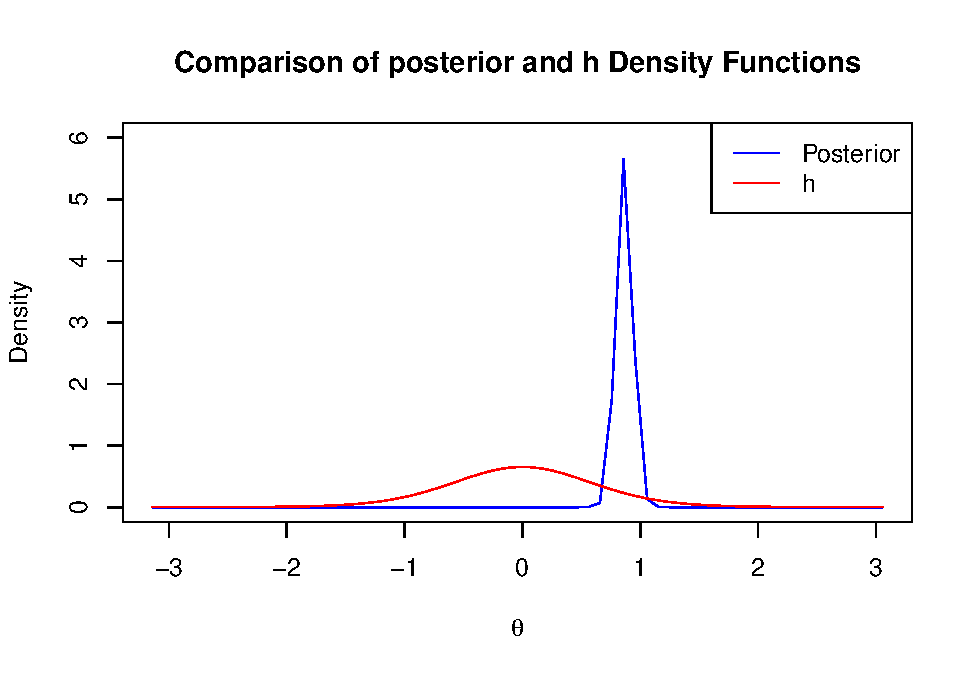
\includegraphics[keepaspectratio]{STA304XS_Ass_1_files/figure-latex/unnamed-chunk-3-1.pdf}}

\begin{Shaded}
\begin{Highlighting}[]
\CommentTok{\# Acceptance{-}Rejection function}
\NormalTok{ar }\OtherTok{\textless{}{-}} \ControlFlowTok{function}\NormalTok{(n) \{}
  
\NormalTok{  samples }\OtherTok{\textless{}{-}} \FunctionTok{numeric}\NormalTok{(}\DecValTok{0}\NormalTok{)}
\NormalTok{  theta\_star }\OtherTok{\textless{}{-}} \FunctionTok{rvonmises}\NormalTok{(n, }\AttributeTok{mu=}\FunctionTok{circular}\NormalTok{(}\DecValTok{0}\NormalTok{), }\AttributeTok{kappa=}\DecValTok{3}\NormalTok{)}
\NormalTok{  u }\OtherTok{\textless{}{-}} \FunctionTok{runif}\NormalTok{(n)}
\NormalTok{  gamma\_vectorised }\OtherTok{\textless{}{-}} \FunctionTok{Vectorize}\NormalTok{(gamma, }\FunctionTok{c}\NormalTok{(}\StringTok{"theta"}\NormalTok{, }\StringTok{"C"}\NormalTok{))}
\NormalTok{  g }\OtherTok{\textless{}{-}} \FunctionTok{gamma\_vectorised}\NormalTok{(theta\_star, C)}
\NormalTok{  accept\_mask }\OtherTok{\textless{}{-}}\NormalTok{ u}\SpecialCharTok{\textless{}}\NormalTok{g}
\NormalTok{  samples }\OtherTok{\textless{}{-}}\NormalTok{ theta\_star[accept\_mask]}
  \FunctionTok{return}\NormalTok{(samples)}
\NormalTok{\}}

\CommentTok{\# Generate posterior draws}
\FunctionTok{set.seed}\NormalTok{(}\DecValTok{123}\NormalTok{)}
\NormalTok{n\_trajectories }\OtherTok{=} \DecValTok{5000}
\NormalTok{samples }\OtherTok{\textless{}{-}} \FunctionTok{ar}\NormalTok{(n\_trajectories)}
\CommentTok{\#samples}
\end{Highlighting}
\end{Shaded}

\begin{enumerate}
\def\labelenumi{(\alph{enumi})}
\setcounter{enumi}{1}
\tightlist
\item
\end{enumerate}

\begin{verbatim}
##        n     Min.  1st Qu.   Median     Mean  3rd Qu.     Max.      Rho 
## 190.0000   0.6460   0.8084   0.8510   0.8579   0.9097   1.1420   0.9968
\end{verbatim}

\begin{verbatim}
## Posterior mean: 0.8578824
\end{verbatim}

\begin{verbatim}
## Posterior sd: 0.07967903
\end{verbatim}

\begin{Shaded}
\begin{Highlighting}[]
\CommentTok{\# Plot posterior}
\FunctionTok{hist}\NormalTok{(}\FunctionTok{as.numeric}\NormalTok{(samples), }\AttributeTok{breaks=} \DecValTok{50}\NormalTok{, }\AttributeTok{freq =} \ConstantTok{FALSE}\NormalTok{,}
     \AttributeTok{col =} \StringTok{"lightblue"}\NormalTok{, }\AttributeTok{main =} \StringTok{"Posterior Distribution of Theta "}\NormalTok{,}
     \AttributeTok{xlab =} \FunctionTok{expression}\NormalTok{(theta))}

\CommentTok{\# Overlay posterior function (rescaled)}
\NormalTok{theta\_grid }\OtherTok{\textless{}{-}} \FunctionTok{seq}\NormalTok{(}\SpecialCharTok{{-}}\NormalTok{pi, pi, }\AttributeTok{length.out =} \DecValTok{200}\NormalTok{)}
\NormalTok{posterior\_vals }\OtherTok{\textless{}{-}} \FunctionTok{sapply}\NormalTok{(theta\_grid,posterior)}
\NormalTok{posterior\_vals }\OtherTok{\textless{}{-}}\NormalTok{ posterior\_vals }\SpecialCharTok{/} \FunctionTok{sum}\NormalTok{(posterior\_vals }\SpecialCharTok{*} \FunctionTok{diff}\NormalTok{(theta\_grid[}\DecValTok{1}\SpecialCharTok{:}\DecValTok{2}\NormalTok{]))  }\CommentTok{\# rescale}
\FunctionTok{lines}\NormalTok{(theta\_grid, posterior\_vals, }\AttributeTok{col =} \StringTok{"red"}\NormalTok{, }\AttributeTok{lwd =} \DecValTok{2}\NormalTok{)}
\end{Highlighting}
\end{Shaded}

\pandocbounded{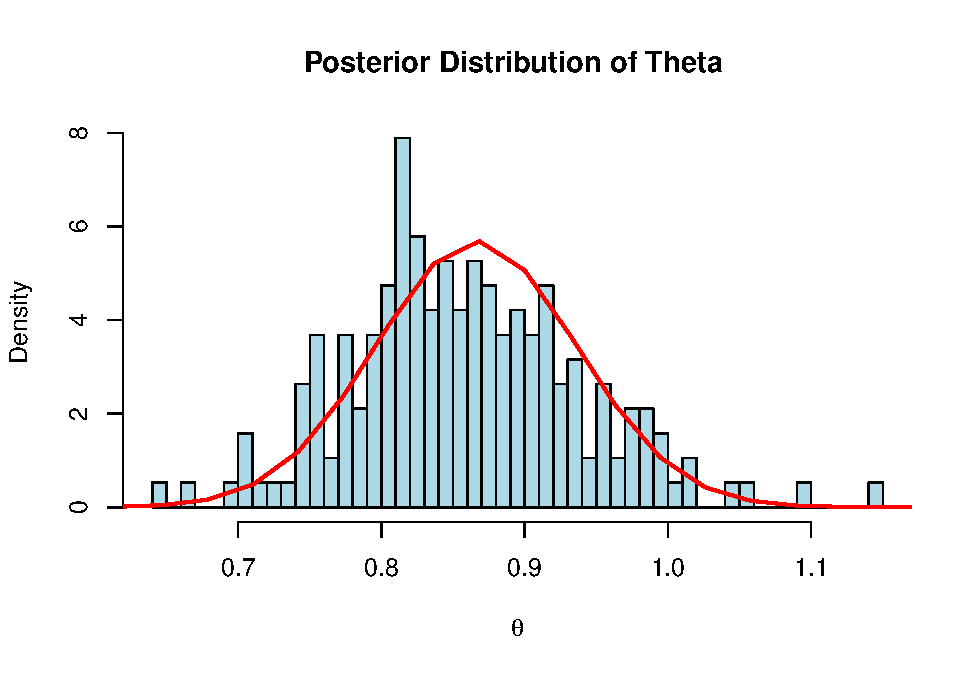
\includegraphics[keepaspectratio]{STA304XS_Ass_1_files/figure-latex/unnamed-chunk-6-1.pdf}}
When plotting posterior samples using hist(\ldots, probability = TRUE)
in R, the histogram is scaled so that the area under the curve sums to
1, approximating a probability density function. The height of the bars
represents the density, not the probability of individual values.
Therefore, if the data are concentrated in a narrow range or if the bin
width is small, the density can exceed 1. This is mathematically valid
because the integral (or sum of bar areas) still equals 1, and the
density value itself is not restricted to be less than or equal to 1. It
simply reflects how concentrated the distribution is over a small
interval.

\subsection{Question 3}\label{question-3}

We use our sample \(\mathbb{\theta}\) to generate a sample of animal
trajectories. Our generated velocities are

\begin{Shaded}
\begin{Highlighting}[]
\FunctionTok{set.seed}\NormalTok{(}\DecValTok{123}\NormalTok{)}
\NormalTok{n\_steps }\OtherTok{=} \DecValTok{252}
\CommentTok{\# To store trajectories}
\NormalTok{V\_mat }\OtherTok{=} \FunctionTok{list}\NormalTok{()}
\NormalTok{MU\_mat }\OtherTok{=} \FunctionTok{list}\NormalTok{()}
\NormalTok{n\_trajectories }\OtherTok{=} \FunctionTok{length}\NormalTok{(samples)}
\ControlFlowTok{for}\NormalTok{ (trial }\ControlFlowTok{in} \DecValTok{1}\SpecialCharTok{:}\NormalTok{n\_trajectories)\{}
\NormalTok{  V\_path }\OtherTok{\textless{}{-}} \FunctionTok{matrix}\NormalTok{(}\DecValTok{0}\NormalTok{, }\AttributeTok{nrow =}\NormalTok{ n\_steps }\SpecialCharTok{+} \DecValTok{1}\NormalTok{, }\AttributeTok{ncol =} \DecValTok{2}\NormalTok{)}
\NormalTok{  MU\_path }\OtherTok{\textless{}{-}} \FunctionTok{matrix}\NormalTok{(}\DecValTok{0}\NormalTok{, }\AttributeTok{nrow =}\NormalTok{ n\_steps }\SpecialCharTok{+} \DecValTok{1}\NormalTok{, }\AttributeTok{ncol =} \DecValTok{2}\NormalTok{)}
\NormalTok{  M }\OtherTok{\textless{}{-}} \FunctionTok{matrix}\NormalTok{(}\FunctionTok{c}\NormalTok{(}\FunctionTok{cos}\NormalTok{(samples[trial]), }\SpecialCharTok{{-}}\FunctionTok{sin}\NormalTok{(samples[trial]),  }\CommentTok{\# Column 1}
                \FunctionTok{sin}\NormalTok{(samples[trial]),  }\FunctionTok{cos}\NormalTok{(samples[trial])),  }\CommentTok{\# Column 2}
              \AttributeTok{nrow =} \DecValTok{2}\NormalTok{)}
\NormalTok{  e\_ }\OtherTok{\textless{}{-}} \FunctionTok{matrix}\NormalTok{(}\FunctionTok{rnorm}\NormalTok{(n\_steps }\SpecialCharTok{*} \DecValTok{2}\NormalTok{), }\AttributeTok{ncol =} \DecValTok{2}\NormalTok{)}
  \ControlFlowTok{for}\NormalTok{ (step }\ControlFlowTok{in} \DecValTok{1}\SpecialCharTok{:}\NormalTok{n\_steps)\{}
\NormalTok{    V\_path[step }\SpecialCharTok{+} \DecValTok{1}\NormalTok{, ] }\OtherTok{\textless{}{-}}  \FloatTok{0.5} \SpecialCharTok{*}\NormalTok{M }\SpecialCharTok{\%*\%}\NormalTok{ V\_path[step,] }\SpecialCharTok{+}\NormalTok{ e\_[step,]}
\NormalTok{    MU\_path[step }\SpecialCharTok{+} \DecValTok{1}\NormalTok{, ] }\OtherTok{=}\NormalTok{ MU\_path[step, ] }\SpecialCharTok{+}\NormalTok{ V\_path[step }\SpecialCharTok{+} \DecValTok{1}\NormalTok{, ]}
\NormalTok{  \}}
\NormalTok{  V\_mat[[trial]] }\OtherTok{\textless{}{-}}\NormalTok{ V\_path}
\NormalTok{  MU\_mat[[trial]] }\OtherTok{\textless{}{-}}\NormalTok{ MU\_path}
\NormalTok{\}}

\NormalTok{final\_positions }\OtherTok{\textless{}{-}} \FunctionTok{t}\NormalTok{(}\FunctionTok{sapply}\NormalTok{(MU\_mat, }\ControlFlowTok{function}\NormalTok{(mat) mat[n\_steps, ]))}

\CommentTok{\# Calculate the mean and variance from these final positions}
\NormalTok{posterior\_mean }\OtherTok{\textless{}{-}} \FunctionTok{colMeans}\NormalTok{(final\_positions)}
\NormalTok{posterior\_variance }\OtherTok{\textless{}{-}} \FunctionTok{cov}\NormalTok{(final\_positions)}

\FunctionTok{cat}\NormalTok{(}\StringTok{"Estimated Posterior Mean of mu\_251:}\SpecialCharTok{\textbackslash{}n}\StringTok{"}\NormalTok{)}
\end{Highlighting}
\end{Shaded}

\begin{verbatim}
## Estimated Posterior Mean of mu_251:
\end{verbatim}

\begin{Shaded}
\begin{Highlighting}[]
\FunctionTok{print}\NormalTok{(posterior\_mean)}
\end{Highlighting}
\end{Shaded}

\begin{verbatim}
## [1] 0.5008737 0.7838762
\end{verbatim}

\begin{Shaded}
\begin{Highlighting}[]
\FunctionTok{cat}\NormalTok{(}\StringTok{"}\SpecialCharTok{\textbackslash{}n}\StringTok{Estimated Posterior Variance of mu\_251:}\SpecialCharTok{\textbackslash{}n}\StringTok{"}\NormalTok{)}
\end{Highlighting}
\end{Shaded}

\begin{verbatim}
## 
## Estimated Posterior Variance of mu_251:
\end{verbatim}

\begin{Shaded}
\begin{Highlighting}[]
\FunctionTok{print}\NormalTok{(posterior\_variance)}
\end{Highlighting}
\end{Shaded}

\begin{verbatim}
##           [,1]      [,2]
## [1,] 395.25557  15.38765
## [2,]  15.38765 362.06679
\end{verbatim}

\subsection{Appendix}\label{appendix}

\begin{Shaded}
\begin{Highlighting}[]
\NormalTok{knitr}\SpecialCharTok{::}\NormalTok{opts\_chunk}\SpecialCharTok{$}\FunctionTok{set}\NormalTok{(}\AttributeTok{echo =} \ConstantTok{TRUE}\NormalTok{)}
\FunctionTok{load}\NormalTok{(}\StringTok{"./STA3043\_Assignment1\_2025.Rdata"}\NormalTok{)}
\NormalTok{data }\OtherTok{\textless{}{-}} \FunctionTok{as.data.frame}\NormalTok{(Class.List[[}\StringTok{"STHSAU001"}\NormalTok{]])}
\NormalTok{mu }\OtherTok{\textless{}{-}} \FunctionTok{cbind}\NormalTok{(data}\SpecialCharTok{$}\NormalTok{x,data}\SpecialCharTok{$}\NormalTok{y)}
\NormalTok{vt }\OtherTok{\textless{}{-}} \FunctionTok{rbind}\NormalTok{(}\FunctionTok{c}\NormalTok{(}\DecValTok{0}\NormalTok{,}\DecValTok{0}\NormalTok{), }\FunctionTok{diff}\NormalTok{(mu))}

\FunctionTok{library}\NormalTok{(circular)}

\NormalTok{n }\OtherTok{\textless{}{-}} \FunctionTok{nrow}\NormalTok{(vt)}


\NormalTok{v\_t1 }\OtherTok{\textless{}{-}}\NormalTok{ vt[}\DecValTok{2}\SpecialCharTok{:}\NormalTok{n, }\DecValTok{1}\NormalTok{]}
\NormalTok{v\_t2 }\OtherTok{\textless{}{-}}\NormalTok{ vt[}\DecValTok{2}\SpecialCharTok{:}\NormalTok{n, }\DecValTok{2}\NormalTok{]}
\NormalTok{v\_tminus1\_1 }\OtherTok{\textless{}{-}}\NormalTok{ vt[}\DecValTok{1}\SpecialCharTok{:}\NormalTok{(n}\DecValTok{{-}1}\NormalTok{), }\DecValTok{1}\NormalTok{]}
\NormalTok{v\_tminus1\_2 }\OtherTok{\textless{}{-}}\NormalTok{ vt[}\DecValTok{1}\SpecialCharTok{:}\NormalTok{(n}\DecValTok{{-}1}\NormalTok{), }\DecValTok{2}\NormalTok{]}
\NormalTok{s1 }\OtherTok{\textless{}{-}} \FunctionTok{sum}\NormalTok{(v\_t1 }\SpecialCharTok{*}\NormalTok{ v\_tminus1\_1 }\SpecialCharTok{+}\NormalTok{ v\_t2 }\SpecialCharTok{*}\NormalTok{ v\_tminus1\_2)}
\NormalTok{s2 }\OtherTok{\textless{}{-}} \FunctionTok{sum}\NormalTok{(v\_t1 }\SpecialCharTok{*}\NormalTok{ v\_tminus1\_2 }\SpecialCharTok{{-}}\NormalTok{ v\_t2 }\SpecialCharTok{*}\NormalTok{ v\_tminus1\_1)}

\CommentTok{\#posterior, same as likelihood, since prior is constant.}
\NormalTok{posterior }\OtherTok{\textless{}{-}} \ControlFlowTok{function}\NormalTok{(theta) \{}
  \FunctionTok{exp}\NormalTok{((s1 }\SpecialCharTok{*} \FunctionTok{cos}\NormalTok{(theta) }\SpecialCharTok{+}\NormalTok{ s2 }\SpecialCharTok{*} \FunctionTok{sin}\NormalTok{(theta))}\SpecialCharTok{/}\DecValTok{2}\NormalTok{)}
\NormalTok{\}}

\CommentTok{\#candidate}
\NormalTok{h }\OtherTok{\textless{}{-}} \ControlFlowTok{function}\NormalTok{(theta) \{}
  \FunctionTok{exp}\NormalTok{(}\DecValTok{3} \SpecialCharTok{*} \FunctionTok{cos}\NormalTok{(theta))}
\NormalTok{\}}


\CommentTok{\# Manual calculation}
\NormalTok{theta\_man }\OtherTok{=} \FunctionTok{atan}\NormalTok{((s2)}\SpecialCharTok{/}\NormalTok{(s1}\DecValTok{{-}6}\NormalTok{))}
\NormalTok{C\_man }\OtherTok{=} \FunctionTok{posterior}\NormalTok{(theta\_man)}\SpecialCharTok{/}\FunctionTok{h}\NormalTok{(theta\_man)}

\CommentTok{\#gamma function}
\NormalTok{gamma }\OtherTok{\textless{}{-}} \ControlFlowTok{function}\NormalTok{(theta, C) \{}
\NormalTok{  (}\FunctionTok{posterior}\NormalTok{(theta)}\SpecialCharTok{/}\NormalTok{(}\FunctionTok{h}\NormalTok{(theta)}\SpecialCharTok{*}\NormalTok{C))}
\NormalTok{\}}
\NormalTok{ opt }\OtherTok{\textless{}{-}} \FunctionTok{optimize}\NormalTok{(}\ControlFlowTok{function}\NormalTok{(theta) }\FunctionTok{posterior}\NormalTok{(theta)}\SpecialCharTok{/}\FunctionTok{h}\NormalTok{(theta),}
                  \AttributeTok{interval =} \FunctionTok{c}\NormalTok{(}\SpecialCharTok{{-}}\NormalTok{pi, pi), }\AttributeTok{maximum =} \ConstantTok{TRUE}\NormalTok{)}
\NormalTok{C }\OtherTok{\textless{}{-}}\NormalTok{ opt}\SpecialCharTok{$}\NormalTok{objective}

\NormalTok{C}
\NormalTok{C\_man}



\NormalTok{kernel }\OtherTok{\textless{}{-}} \ControlFlowTok{function}\NormalTok{(theta, kappa, mean) \{}
  \FunctionTok{return}\NormalTok{ (}\FunctionTok{exp}\NormalTok{(kappa }\SpecialCharTok{*} \FunctionTok{cos}\NormalTok{(theta }\SpecialCharTok{{-}}\NormalTok{ mean)));}
\NormalTok{\};}

\NormalTok{vonMises\_density }\OtherTok{\textless{}{-}} \ControlFlowTok{function}\NormalTok{(theta, kappa, mean) \{}
  \FunctionTok{return}\NormalTok{ (}\FunctionTok{kernel}\NormalTok{(theta, kappa, mean) }\SpecialCharTok{/} \FunctionTok{integrate}\NormalTok{(kernel, }\AttributeTok{lower=}\SpecialCharTok{{-}}\NormalTok{pi, }\AttributeTok{upper=}\NormalTok{pi, }\AttributeTok{kappa=}\NormalTok{kappa, }\AttributeTok{mean=}\NormalTok{mean)}\SpecialCharTok{$}\NormalTok{value)}
\NormalTok{\}}

\NormalTok{posterior\_normalised }\OtherTok{\textless{}{-}} \ControlFlowTok{function}\NormalTok{(theta)\{}
  \FunctionTok{return}\NormalTok{ (}\FunctionTok{posterior}\NormalTok{(theta) }\SpecialCharTok{/} \FunctionTok{integrate}\NormalTok{(posterior, }\AttributeTok{lower=}\SpecialCharTok{{-}}\NormalTok{pi, }\AttributeTok{upper=}\NormalTok{pi)}\SpecialCharTok{$}\NormalTok{value)}
\NormalTok{\}}

\NormalTok{theta }\OtherTok{\textless{}{-}} \FunctionTok{seq}\NormalTok{(}\SpecialCharTok{{-}}\NormalTok{pi, pi, }\FloatTok{0.1}\NormalTok{)}
\NormalTok{posterior\_vectorised }\OtherTok{\textless{}{-}} \FunctionTok{Vectorize}\NormalTok{(posterior\_normalised)}
\NormalTok{vonMises\_vectorised }\OtherTok{\textless{}{-}} \FunctionTok{Vectorize}\NormalTok{(vonMises\_density, }\StringTok{"theta"}\NormalTok{)}

\CommentTok{\# Plot the first function}
\FunctionTok{plot}\NormalTok{(theta, }\FunctionTok{posterior\_vectorised}\NormalTok{(theta),}
     \AttributeTok{type =} \StringTok{"l"}\NormalTok{,}
     \AttributeTok{col =} \StringTok{"blue"}\NormalTok{,}
     \AttributeTok{ylim =} \FunctionTok{c}\NormalTok{(}\DecValTok{0}\NormalTok{, }\DecValTok{6}\NormalTok{),}
     \AttributeTok{xlab =} \FunctionTok{expression}\NormalTok{(theta),}
     \AttributeTok{ylab =} \StringTok{"Density"}\NormalTok{,}
     \AttributeTok{main =} \StringTok{"Comparison of posterior and h Density Functions"}\NormalTok{)}

\CommentTok{\# Add the second function to the same plot}
\FunctionTok{lines}\NormalTok{(theta, }\FunctionTok{vonMises\_vectorised}\NormalTok{(theta, }\DecValTok{3}\NormalTok{, }\DecValTok{0}\NormalTok{) , }\AttributeTok{col =} \StringTok{"red"}\NormalTok{)}

\CommentTok{\# Add a legend to distinguish the lines}
\FunctionTok{legend}\NormalTok{(}\StringTok{"topright"}\NormalTok{,}
       \AttributeTok{legend =} \FunctionTok{c}\NormalTok{(}\StringTok{"Posterior"}\NormalTok{, }\StringTok{"h"}\NormalTok{),}
       \AttributeTok{col =} \FunctionTok{c}\NormalTok{(}\StringTok{"blue"}\NormalTok{, }\StringTok{"red"}\NormalTok{),}
       \AttributeTok{lty =} \DecValTok{1}\NormalTok{)}
\CommentTok{\# Acceptance{-}Rejection function}
\NormalTok{ar }\OtherTok{\textless{}{-}} \ControlFlowTok{function}\NormalTok{(n) \{}
  
\NormalTok{  samples }\OtherTok{\textless{}{-}} \FunctionTok{numeric}\NormalTok{(}\DecValTok{0}\NormalTok{)}
\NormalTok{  theta\_star }\OtherTok{\textless{}{-}} \FunctionTok{rvonmises}\NormalTok{(n, }\AttributeTok{mu=}\FunctionTok{circular}\NormalTok{(}\DecValTok{0}\NormalTok{), }\AttributeTok{kappa=}\DecValTok{3}\NormalTok{)}
\NormalTok{  u }\OtherTok{\textless{}{-}} \FunctionTok{runif}\NormalTok{(n)}
\NormalTok{  gamma\_vectorised }\OtherTok{\textless{}{-}} \FunctionTok{Vectorize}\NormalTok{(gamma, }\FunctionTok{c}\NormalTok{(}\StringTok{"theta"}\NormalTok{, }\StringTok{"C"}\NormalTok{))}
\NormalTok{  g }\OtherTok{\textless{}{-}} \FunctionTok{gamma\_vectorised}\NormalTok{(theta\_star, C)}
\NormalTok{  accept\_mask }\OtherTok{\textless{}{-}}\NormalTok{ u}\SpecialCharTok{\textless{}}\NormalTok{g}
\NormalTok{  samples }\OtherTok{\textless{}{-}}\NormalTok{ theta\_star[accept\_mask]}
  \FunctionTok{return}\NormalTok{(samples)}
\NormalTok{\}}

\CommentTok{\# Generate posterior draws}
\FunctionTok{set.seed}\NormalTok{(}\DecValTok{123}\NormalTok{)}
\NormalTok{n\_trajectories }\OtherTok{=} \DecValTok{5000}
\NormalTok{samples }\OtherTok{\textless{}{-}} \FunctionTok{ar}\NormalTok{(n\_trajectories)}
\CommentTok{\#samples}
\CommentTok{\# Posterior summaries}
\FunctionTok{summary}\NormalTok{(samples)}
\FunctionTok{cat}\NormalTok{(}\StringTok{"Posterior mean:"}\NormalTok{, }\FunctionTok{mean}\NormalTok{(samples), }\StringTok{"}\SpecialCharTok{\textbackslash{}n}\StringTok{"}\NormalTok{)}
\FunctionTok{cat}\NormalTok{(}\StringTok{"Posterior sd:"}\NormalTok{, }\FunctionTok{sd}\NormalTok{(samples), }\StringTok{"}\SpecialCharTok{\textbackslash{}n}\StringTok{"}\NormalTok{)}

\CommentTok{\# Plot posterior}
\FunctionTok{hist}\NormalTok{(}\FunctionTok{as.numeric}\NormalTok{(samples), }\AttributeTok{breaks=} \DecValTok{50}\NormalTok{, }\AttributeTok{freq =} \ConstantTok{FALSE}\NormalTok{,}
     \AttributeTok{col =} \StringTok{"lightblue"}\NormalTok{, }\AttributeTok{main =} \StringTok{"Posterior Distribution of Theta "}\NormalTok{,}
     \AttributeTok{xlab =} \FunctionTok{expression}\NormalTok{(theta))}

\CommentTok{\# Overlay posterior function (rescaled)}
\NormalTok{theta\_grid }\OtherTok{\textless{}{-}} \FunctionTok{seq}\NormalTok{(}\SpecialCharTok{{-}}\NormalTok{pi, pi, }\AttributeTok{length.out =} \DecValTok{200}\NormalTok{)}
\NormalTok{posterior\_vals }\OtherTok{\textless{}{-}} \FunctionTok{sapply}\NormalTok{(theta\_grid,posterior)}
\NormalTok{posterior\_vals }\OtherTok{\textless{}{-}}\NormalTok{ posterior\_vals }\SpecialCharTok{/} \FunctionTok{sum}\NormalTok{(posterior\_vals }\SpecialCharTok{*} \FunctionTok{diff}\NormalTok{(theta\_grid[}\DecValTok{1}\SpecialCharTok{:}\DecValTok{2}\NormalTok{]))  }\CommentTok{\# rescale}
\FunctionTok{lines}\NormalTok{(theta\_grid, posterior\_vals, }\AttributeTok{col =} \StringTok{"red"}\NormalTok{, }\AttributeTok{lwd =} \DecValTok{2}\NormalTok{)}

\FunctionTok{set.seed}\NormalTok{(}\DecValTok{123}\NormalTok{)}
\NormalTok{n\_steps }\OtherTok{=} \DecValTok{252}
\CommentTok{\# To store trajectories}
\NormalTok{V\_mat }\OtherTok{=} \FunctionTok{list}\NormalTok{()}
\NormalTok{MU\_mat }\OtherTok{=} \FunctionTok{list}\NormalTok{()}
\NormalTok{n\_trajectories }\OtherTok{=} \FunctionTok{length}\NormalTok{(samples)}
\ControlFlowTok{for}\NormalTok{ (trial }\ControlFlowTok{in} \DecValTok{1}\SpecialCharTok{:}\NormalTok{n\_trajectories)\{}
\NormalTok{  V\_path }\OtherTok{\textless{}{-}} \FunctionTok{matrix}\NormalTok{(}\DecValTok{0}\NormalTok{, }\AttributeTok{nrow =}\NormalTok{ n\_steps }\SpecialCharTok{+} \DecValTok{1}\NormalTok{, }\AttributeTok{ncol =} \DecValTok{2}\NormalTok{)}
\NormalTok{  MU\_path }\OtherTok{\textless{}{-}} \FunctionTok{matrix}\NormalTok{(}\DecValTok{0}\NormalTok{, }\AttributeTok{nrow =}\NormalTok{ n\_steps }\SpecialCharTok{+} \DecValTok{1}\NormalTok{, }\AttributeTok{ncol =} \DecValTok{2}\NormalTok{)}
\NormalTok{  M }\OtherTok{\textless{}{-}} \FunctionTok{matrix}\NormalTok{(}\FunctionTok{c}\NormalTok{(}\FunctionTok{cos}\NormalTok{(samples[trial]), }\SpecialCharTok{{-}}\FunctionTok{sin}\NormalTok{(samples[trial]),  }\CommentTok{\# Column 1}
                \FunctionTok{sin}\NormalTok{(samples[trial]),  }\FunctionTok{cos}\NormalTok{(samples[trial])),  }\CommentTok{\# Column 2}
              \AttributeTok{nrow =} \DecValTok{2}\NormalTok{)}
\NormalTok{  e\_ }\OtherTok{\textless{}{-}} \FunctionTok{matrix}\NormalTok{(}\FunctionTok{rnorm}\NormalTok{(n\_steps }\SpecialCharTok{*} \DecValTok{2}\NormalTok{), }\AttributeTok{ncol =} \DecValTok{2}\NormalTok{)}
  \ControlFlowTok{for}\NormalTok{ (step }\ControlFlowTok{in} \DecValTok{1}\SpecialCharTok{:}\NormalTok{n\_steps)\{}
\NormalTok{    V\_path[step }\SpecialCharTok{+} \DecValTok{1}\NormalTok{, ] }\OtherTok{\textless{}{-}}  \FloatTok{0.5} \SpecialCharTok{*}\NormalTok{M }\SpecialCharTok{\%*\%}\NormalTok{ V\_path[step,] }\SpecialCharTok{+}\NormalTok{ e\_[step,]}
\NormalTok{    MU\_path[step }\SpecialCharTok{+} \DecValTok{1}\NormalTok{, ] }\OtherTok{=}\NormalTok{ MU\_path[step, ] }\SpecialCharTok{+}\NormalTok{ V\_path[step }\SpecialCharTok{+} \DecValTok{1}\NormalTok{, ]}
\NormalTok{  \}}
\NormalTok{  V\_mat[[trial]] }\OtherTok{\textless{}{-}}\NormalTok{ V\_path}
\NormalTok{  MU\_mat[[trial]] }\OtherTok{\textless{}{-}}\NormalTok{ MU\_path}
\NormalTok{\}}

\NormalTok{final\_positions }\OtherTok{\textless{}{-}} \FunctionTok{t}\NormalTok{(}\FunctionTok{sapply}\NormalTok{(MU\_mat, }\ControlFlowTok{function}\NormalTok{(mat) mat[n\_steps, ]))}

\CommentTok{\# Calculate the mean and variance from these final positions}
\NormalTok{posterior\_mean }\OtherTok{\textless{}{-}} \FunctionTok{colMeans}\NormalTok{(final\_positions)}
\NormalTok{posterior\_variance }\OtherTok{\textless{}{-}} \FunctionTok{cov}\NormalTok{(final\_positions)}

\FunctionTok{cat}\NormalTok{(}\StringTok{"Estimated Posterior Mean of mu\_251:}\SpecialCharTok{\textbackslash{}n}\StringTok{"}\NormalTok{)}
\FunctionTok{print}\NormalTok{(posterior\_mean)}

\FunctionTok{cat}\NormalTok{(}\StringTok{"}\SpecialCharTok{\textbackslash{}n}\StringTok{Estimated Posterior Variance of mu\_251:}\SpecialCharTok{\textbackslash{}n}\StringTok{"}\NormalTok{)}
\FunctionTok{print}\NormalTok{(posterior\_variance)}
\end{Highlighting}
\end{Shaded}







\end{document}
